\documentclass{article}
\usepackage{amsmath}
\usepackage{amssymb}
\usepackage{enumitem}
\usepackage{fancyvrb}
\usepackage{booktabs}
\usepackage{tikz}
\usepackage{graphicx}
\usetikzlibrary{graphs}
\usepackage[utf8]{inputenc}
\usepackage[T5]{fontenc}
\usepackage[vietnamese]{babel}

\title{Combinatorics And Graph Theory-Final}
\author{Phạm Phước Minh Hiếu}

\begin{document}
	\section*{Project 1: Mathematical Induction {\it\&} Recurrence Relations -- Đồ Án 1: Quy Nạp Toán Học {\it\&} Quan Hệ Truy Hồi}
	
	\subsection{Mathematical Induction -- Quy nạp toán học}
	
	\textbf{Định lý.} Với mọi $n \in \mathbb{N},\ n \ge 1$, ta có:
	\[
	\sum_{k=1}^{n} k = \frac{n(n+1)}{2}.
	\]
	
	\textbf{Chứng minh:} Sử dụng phương pháp quy nạp toán học.
	
	\begin{itemize}[leftmargin=1.5cm]
		\item \textbf{Cơ sở quy nạp:} Với $n = 1$:
		\[
		\sum_{k=1}^{1} k = 1 = \frac{1(1+1)}{2} = 1.
		\]
		Đúng.
		
		\item \textbf{Giả thiết quy nạp:} Giả sử công thức đúng với $n = k$, tức là:
		\[
		\sum_{i=1}^{k} i = \frac{k(k+1)}{2}.
		\]
		
		\item \textbf{Bước quy nạp:} Xét $n = k + 1$:
		\begin{align*}
			\sum_{i=1}^{k+1} i &= \left(\sum_{i=1}^{k} i\right) + (k+1) \\
			&= \frac{k(k+1)}{2} + (k+1) \quad \text{(theo giả thiết quy nạp)}\\
			&= \frac{k(k+1) + 2(k+1)}{2} \\
			&= \frac{(k+1)(k + 2)}{2}.
		\end{align*}
		Đây chính là công thức với $n = k + 1$.
		
		\item \textbf{Kết luận:} Theo nguyên lý quy nạp, mệnh đề được chứng minh đúng với mọi $n \in \mathbb{N},\ n \ge 1$.
	\end{itemize}
	
	\subsection{Recurrence Relation -- Quan hệ truy hồi}
	
	\textbf{Đề bài:} Xét dãy truy hồi:
	\[
	a_1 = 1,\quad a_n = a_{n-1} + 2n - 1 \quad \text{với } n \ge 2.
	\]
	
	\textbf{Tìm công thức tổng quát của $a_n$ theo $n$.}
	
	\textbf{Giải:}
	
	Ta tính một vài giá trị đầu:
	\[
	a_1 = 1,\quad a_2 = 1 + 3 = 4,\quad a_3 = 4 + 5 = 9,\quad a_4 = 9 + 7 = 16.
	\]
	
	Dễ thấy:
	\[
	a_n = n^2.
	\]
	
	\textbf{Chứng minh bằng quy nạp:}
	
	\begin{itemize}[leftmargin=1.5cm]
		\item \textbf{Cơ sở:} $n = 1$: $a_1 = 1 = 1^2$, đúng.
		
		\item \textbf{Giả thiết quy nạp:} Giả sử $a_k = k^2$ đúng với một $k \ge 1$.
		
		\item \textbf{Bước quy nạp:}
		\[
		a_{k+1} = a_k + 2(k+1) - 1 = k^2 + 2k + 1 = (k+1)^2.
		\]
		
		\item \textbf{Kết luận:} $a_n = n^2$ với mọi $n \in \mathbb{N},\ n \ge 1$.
	\end{itemize}
	
	\section*{Project 2: Counting, Probability, Balls, \& Boxes -- Đồ Án 2: Đếm, Xác Suất, Banh \& Hộp}
	
	\textbf{Cho 5 quả banh phân biệt và 3 hộp phân biệt.}
	
	\begin{itemize}[leftmargin=1.5cm]
		\item[(a)] Có bao nhiêu cách đặt 5 quả banh vào 3 hộp?
		\item[(b)] Nếu mỗi quả banh được đặt ngẫu nhiên vào một hộp (các quả độc lập, xác suất như nhau), xác suất có ít nhất một hộp trống là bao nhiêu?
	\end{itemize}
	
	\subsection*{Câu (a):}
	Mỗi quả banh có 3 lựa chọn để vào một trong 3 hộp.
	
	Vì các quả banh là phân biệt và được đặt độc lập:
	\[
	\text{Tổng số cách} = 3^5 = 243.
	\]
	
	\subsection*{Câu (b):}
	Ta cần tính:
	\[
	\mathbb{P}(\text{ít nhất một hộp trống}) = 1 - \mathbb{P}(\text{không có hộp nào trống}).
	\]
	
	\textbf{Gọi $A$ là biến cố “không có hộp nào trống”}
	
	Áp dụng nguyên lý bao hàm – loại trừ (Inclusion–Exclusion), ta tính số cách phân chia 5 quả banh (phân biệt) vào 3 hộp (phân biệt) sao cho mỗi hộp có ít nhất 1 quả (không rỗng).
	
	Số cách:
	\[
	N = 3^5 - \binom{3}{1} 2^5 + \binom{3}{2} 1^5 = 243 - 3 \cdot 32 + 3 \cdot 1 = 243 - 96 + 3 = 150.
	\]
	
	Vậy xác suất để không hộp nào trống là:
	\[
	\mathbb{P}(A) = \frac{150}{243}.
	\]
	
	Vậy xác suất có ít nhất một hộp trống:
	\[
	1 - \frac{150}{243} = \frac{93}{243} = \frac{31}{81} \approx 0.38
	\]
	
	\section*{Project 3: Generating Functions -- Đồ Án 3: Hàm Sinh}
	
	\textbf{Cho 1 ví dụ:}
		Cho vô hạn số đồng xu có mệnh giá: 1, 2 và 5.  
	Hỏi có bao nhiêu cách chọn các đồng xu (không giới hạn số lượng mỗi loại) để tổng tiền bằng 10?
	
	\subsection*{Hàm sinh của từng loại đồng xu:}
	
	\begin{itemize}
		\item Với đồng xu 1: $1 + x + x^2 + x^3 + \cdots = \dfrac{1}{1 - x}$  
		\item Với đồng xu 2: $1 + x^2 + x^4 + x^6 + \cdots = \dfrac{1}{1 - x^2}$
		\item Với đồng xu 5: $1 + x^5 + x^{10} + x^{15} + \cdots = \dfrac{1}{1 - x^5}$
	\end{itemize}
	
	\subsection*{Hàm sinh tổng hợp:}
	
	Hàm sinh đếm số cách chọn các đồng xu để tổng là $n$:
	\[
	G(x) = \frac{1}{(1 - x)(1 - x^2)(1 - x^5)}
	\]
	
	Ta cần tìm hệ số của $x^{10}$ trong khai triển của $G(x)$:
	\[
	[x^{10}]\,G(x) = ?
	\]
	
	Với $[x^{10}]$:
	
	Ta sẽ đếm số cách chọn bộ số \((a, b, c)\) nguyên không âm sao cho:
	\[
	a + 2b + 5c = 10.
	\]
	
	\noindent\textbf{Trường hợp \(c = 0\):} \(a + 2b = 10\)
	
	\begin{itemize}[leftmargin=1.5cm]
		\item \(b = 0 \Rightarrow a = 10\)
		\item \(b = 1 \Rightarrow a = 8\)
		\item \(b = 2 \Rightarrow a = 6\)
		\item \(b = 3 \Rightarrow a = 4\)
		\item \(b = 4 \Rightarrow a = 2\)
		\item \(b = 5 \Rightarrow a = 0\)
	\end{itemize}
	Có \textbf{6 cách}.
	
	\noindent\textbf{Trường hợp \(c = 1\):} \(a + 2b = 5\)
	
	\begin{itemize}[leftmargin=1.5cm]
		\item \(b = 0 \Rightarrow a = 5\)
		\item \(b = 1 \Rightarrow a = 3\)
		\item \(b = 2 \Rightarrow a = 1\)
	\end{itemize}
	Có \textbf{3 cách}.
	
	\noindent\textbf{Trường hợp \(c = 2\):} \(a + 2b = 0\) \\
	Chỉ có 1 nghiệm: \(a = 0, b = 0\)
	
	\subsection*{3.2. Tổng số cách}
	
	Tổng cộng có:
	\[
	6 + 3 + 1 = \boxed{10} \text{ cách}.
	\]
	
	$\Rightarrow [x^{10}]\,G(x) = 10.$
	
	\section*{Project: Integer Partition -- Đồ Án: Phân Hoạch Số Nguyên}
	
	\subsection*{\underline{Bài toán 1:} Ferrers \& Ferrers transpose diagrams -- Biểu đồ Ferrers \& biểu đồ Ferrers chuyển vị}
	
	Nhập $n,k\in\mathbb{N}$. Viết chương trình {\sf C{\tt/}C++, Python} để in ra $p_k(n)$ biểu đồ Ferrers $F$ \& biểu đồ Ferrers chuyển vị $F^\top$ cho mỗi phân hoạch $\boldsymbol{\lambda} = (\lambda_1,\lambda_2,\ldots,\lambda_k)\in(\mathbb{N}^\star)^k$ có định dạng các dấu chấm được biểu diễn bởi dấu {\tt*}.
	
	\textbf{Ví dụ:}
	
	Cho $n = 5$, $k = 2$. Các phân hoạch của 5 thành đúng 2 phần tử là:
	
	\begin{itemize}
		\item $(4,1)$
		\item $(3,2)$
	\end{itemize}
	
	Biểu diễn Ferrers và Ferrers chuyển vị:
	
	\subsubsection*{Phân hoạch $(4,1)$}
	
	\textbf{Ferrers:}
	\begin{Verbatim}
		****
		*
	\end{Verbatim}
	
	\textbf{Ferrers chuyển vị:}
	\begin{Verbatim}
		**
		*
		*
		*
	\end{Verbatim}
	
	\subsubsection*{Phân hoạch $(3,2)$}
	
	\textbf{Ferrers:}
	\begin{Verbatim}
		***
		**
	\end{Verbatim}
	
	\textbf{Ferrers chuyển vị:}
	\begin{Verbatim}
		**
		**
		*
	\end{Verbatim}
	
	\subsection*{\underline{Bài toán 2:} Nhập $n,k\in\mathbb{N}$. Đếm số phân hoạch của $n\in\mathbb{N}$. Viết chương trình {\sf C{\tt/}C++, Python} để đếm số phân hoạch $p_{\max}(n,k)$ của $n$ sao cho phần tử lớn nhất là $k$. So sánh $p_k(n)$ \& $p_{\max}(n,k)$.
	}
	
	\textbf{Theo đề bài:} Cho $n, k \in \mathbb{N}$. Đếm:
	\begin{itemize}
		\item $p_k(n)$: số phân hoạch của $n$ thành đúng $k$ số nguyên dương.
		\item $p_{\max}(n, k)$: số phân hoạch của $n$ sao cho phần tử lớn nhất đúng bằng $k$.
	\end{itemize}
	
	\textbf{Cho một ví dụ với $n=5$}
	
	\begin{itemize}
		\item Các phân hoạch thành đúng $k=2$ phần tử:
		\[
		(4,1), (3,2)
		\quad\Rightarrow\quad p_2(5) = 2
		\]
		\item Các phân hoạch của $n=5$ có phần tử lớn nhất là $k=2$:
		\[
		(2,2,1), (2,1,1,1), (1,1,1,1,1)
		\quad\Rightarrow\quad p_{\max}(5,2) = 3
		\]
	\end{itemize}
	
	\[
	p_2(5) = 2 \quad\text{vs.}\quad p_{\max}(5,2) = 3
	\]
	\newpage
	\textbf{Thử so sánh với $p_2$(n) và $p_{max}$(n,2)}
	\begin{center}
		\begin{tabular}{@{}ccc@{}}
			\toprule
			$n$ & $p_2(n)$ & $p_{\max}(n,2)$ \\
			\midrule
			1 & 0 & 0 \\
			2 & 1 & 1 \\
			3 & 1 & 1 \\
			4 & 2 & 2 \\
			5 & 2 & 3 \\
			6 & 3 & 4 \\
			\bottomrule
		\end{tabular}
	\end{center}
	
	\subsection*{Số phân hoạch tự liên hợp}
	 Nhập $n,k\in\mathbb{N}$. 
	 \begin{itemize}
	 	\item (a) Đếm số phân hoạch tự liên hợp của $n$ có $k$ phần, ký hiệu $p_k^{\rm selfcjg}(n)$, rồi in ra các phân hoạch đó.
	 	\item (b) Đếm số phân hoạch của $n$ có lẻ phần, rồi so sánh với $p_k^{\rm selfcjg}(n)$.
	 	\item (c) Thiết lập công thức truy hồi cho $p_k^{\rm selfcjg}(n)$, rồi implementation bằng: (i) đệ quy. (ii) quy hoạch động.
	 \end{itemize}
	   
	Cho $n,k\in\mathbb{N}$.
	
	\begin{itemize}
		\item[(a)] Đếm số phân hoạch tự liên hợp của $n$ có đúng $k$ phần, ký hiệu là $p_k^{\text{selfcjg}}(n)$ và liệt kê các phân hoạch đó.
		
		\textbf{Ví dụ:} Với $n=7$, các phân hoạch tự liên hợp gồm: 
		\[
		(4,3),\quad (3,3,1),\quad (2,2,2,1),\quad (1,1,1,1,1,1,1)
		\]
		Khi lọc theo số phần $k$, ta chỉ giữ các phân hoạch có đúng $k$ phần tử.
		
		\item[(b)] Đếm số phân hoạch của $n$ có số phần tử là số lẻ. So sánh giá trị đó với $p_k^{\text{selfcjg}}(n)$.  
		Ký hiệu tổng số phân hoạch có số phần lẻ là $q(n)$.
		
		\textbf{Định lý:} Tổng số phân hoạch tự liên hợp của $n$ đúng bằng số phân hoạch có số phần tử lẻ (Euler).
		
		\item[(c)] \textbf{Thiết lập công thức truy hồi cho $p_k^{\text{selfcjg}}(n)$}
		
		Gọi $p_k^{\text{selfcjg}}(n)$ là số phân hoạch \textbf{tự liên hợp} của $n$ thành đúng $k$ phần.
		
		Do một phân hoạch tự liên hợp luôn gồm các số lẻ không tăng và không vượt quá $k$, do đối xứng qua đường chéo chính của biểu đồ Ferrers.
		
		Ta có thể định nghĩa truy hồi như sau:
		
		\[
		p_k^{\text{selfcjg}}(n) =
		\begin{cases}
			1, & \text{nếu } n = 0 \text{ và } k = 0 \\
			0, & \text{nếu } n < 0 \text{ hoặc } k \leq 0 \\
			\sum\limits_{\substack{1 \leq m \leq \min(2k-1,n)\\ m \text{ lẻ}}} p_{k-1}^{\text{selfcjg}}(n - m), & \text{ngược lại}
		\end{cases}
		\]
		
		
		$\rightarrow$ Mỗi phần thêm vào là một số lẻ $m$, ta trừ nó khỏi $n$ và giảm số phần đi 1.
		
		$\rightarrow$ Ràng buộc số lẻ xuất hiện là do cấu trúc đối xứng: mỗi điểm ở trên đường chéo cần đối xứng với một điểm dưới đường chéo, nên số phần tử ở mỗi dòng phải lẻ.
		
		\textbf{Ngoài ra}, ta có thể thiết lập công thức không phụ thuộc vào $k$, khi đếm tổng số phân hoạch tự liên hợp (tức là $p^{\text{selfcjg}}(n) = \sum_k p_k^{\text{selfcjg}}(n)$):
		
		\[
		p^{\text{selfcjg}}(n) = \# \left\{ (\lambda_1, \lambda_2, \dots, \lambda_k) \mid \sum_{i=1}^k \lambda_i = n,\ \lambda_i \text{ lẻ},\ \lambda_1 \geq \lambda_2 \geq \cdots \geq \lambda_k,\ \lambda_i \geq i \right\}
		\]
		
		Trong đó điều kiện \( \lambda_i \geq i \) đảm bảo đối xứng qua đường chéo chính.
		
		\textbf{Công thức tạo hàm sinh:} Hàm sinh của số phân hoạch tự liên hợp là:
		
		\[
		\sum_{n=0}^\infty p^{\text{selfcjg}}(n) q^n = \prod_{k=1}^\infty (1 + q^{2k-1})
		\]
		
		Do mỗi phần tử trong phân hoạch tự liên hợp tương ứng với một chiều dài móc câu (hook length) lẻ.
		
		
	\end{itemize}
	
	\section*{Project 4: Graph \& Tree Traversing Problems -- Đồ Án 4: Các Bài Toán Duyệt Đồ Thị \& Cây}
	
	\subsection*{Viết chương trình {\sf C{\tt/}C++, Python} chuyển đổi giữa 4 dạng biểu diễn: adjacency matrix, adjacency list, extended adjacency list, adjacency map cho $3$ đồ thị: đơn đồ thị, đa đồ thị, đồ thị tổng quát; \& 3 dạng biểu diễn: array of parents, first-child next-sibling, graph-based representation of trees của cây.}
	
	Sẽ có $3A_4^3 + A_3^2 = 36 + 6 = 42$ converter programs.

	\subsection*{Làm Problems 1.1--1.6 \& Exercises 1.1--1.10.}
	
	\subsubsection*{1.1  Determine the size of the complete graph Kn on n vertices and the complete bipartite graph Kp,q on p + q vertices.}
	
	\paragraph*{1.1.1. Đồ thị đầy đủ \( K_n \):}
	
	Đồ thị đầy đủ \( K_n \) là đồ thị đơn vô hướng trong đó mỗi cặp hai đỉnh phân biệt đều được nối với nhau bởi đúng một cạnh.
	
	Tổng số cạnh trong \( K_n \) chính là số cách chọn ra 2 đỉnh bất kỳ từ \( n \) đỉnh để nối thành một cạnh:
	\[
	\text{Số cạnh của } K_n = \binom{n}{2} = \frac{n(n-1)}{2}
	\]
	
	\paragraph*{1.1.2. Đồ thị hai phía đầy đủ \( K_{p,q} \):}
	
	Đồ thị hai phía đầy đủ \( K_{p,q} \) là đồ thị trong đó tập đỉnh được chia thành hai tập rời \( V_1 \) và \( V_2 \) với kích thước lần lượt là \( p \) và \( q \), và mỗi đỉnh trong \( V_1 \) được nối với mọi đỉnh trong \( V_2 \).
	
	Do đó, tổng số cạnh là:
	\[
	\text{Số cạnh của } K_{p,q} = p \cdot q
	\]
	
	\subsubsection*{1.2 Determine the values of n for which the circle graph Cn on n vertices is bipartite,  and also the values of n for which the complete graph Kn is bipartite.}
	
	\paragraph*{1.2.1. Đồ thị vòng \( C_n \):}
	
	Đồ thị vòng \( C_n \) là một đồ thị mà các đỉnh được nối thành một vòng khép kín. Một đồ thị là hai phía khi và chỉ khi nó không chứa chu trình lẻ.
	
	Như vậy: \( C_n \) chỉ chứa một chu trình có độ dài đúng bằng \( n \), nên:
	\begin{itemize}
		\item Nếu \( n \) chẵn thì \( C_n \) không chứa chu trình lẻ \( \Rightarrow \) là đồ thị hai phía.
		\item Nếu \( n \) lẻ thì \( C_n \) chứa chu trình lẻ \( \Rightarrow \) không là đồ thị hai phía.
	\end{itemize}
	
	$\rightarrow$ \( C_n \) là đồ thị hai phía khi và chỉ khi \( n \) là số chẵn:
	\[
	\boxed{C_n \text{ là đồ thị hai phía khi } n \equiv 0 \pmod{2}}
	\]
	
	\paragraph*{1.2.2. Đồ thị đầy đủ \( K_n \):}
	
	Đồ thị đầy đủ \( K_n \) là đồ thị mà mỗi cặp hai đỉnh phân biệt đều được nối bởi một cạnh.
	
	Như vậy: một đồ thị hai phía không thể chứa tam giác (chu trình độ dài 3), nhưng \( K_n \) với \( n \geq 3 \) luôn chứa tam giác (vì mọi bộ ba đỉnh bất kỳ đều tạo thành một tam giác).
	
	\begin{itemize}
		\item Với \( n = 1 \): \( K_1 \) không có cạnh nào, nên là đồ thị hai phía.
		\item Với \( n = 2 \): \( K_2 \) chỉ có 1 cạnh nối 2 đỉnh, rõ ràng là hai phía.
		\item Với \( n \geq 3 \): \( K_n \) chứa chu trình lẻ (tam giác), nên không phải hai phía.
	\end{itemize}
	
	Do đó: $K_n$ \text{ là đồ thị hai phía khi và chỉ khi } n $\leq$ 2
	
	\subsubsection*{1.3 Give all the spanning trees of the graph in Fig. 1.30, and also the number of spanning trees of the underlying undirected graph.}
	
	\begin{center}
	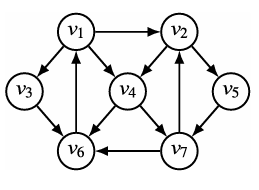
\includegraphics[width=4cm, height=3cm]{Images/1_30.png}
	\end{center}
	
	\textbf{Bước 1: Chuyển sang đồ thị vô hướng}
	
	Ta bỏ hướng của tất cả các cung trong Hình 1.30 để thu được đồ thị vô hướng tương ứng. Tập các cạnh vô hướng là:
	
	\[
	\begin{aligned}
		E = \{ 
		& \{v_1, v_2\},\ \{v_1, v_4\},\ \{v_1, v_6\}, \\
		& \{v_2, v_4\},\ \{v_2, v_5\}, \\
		& \{v_3, v_1\},\ \{v_3, v_6\}, \\
		& \{v_4, v_6\},\ \{v_4, v_7\}, \\
		& \{v_6, v_7\} 
		\}
	\end{aligned}
	\]
	
	Số đỉnh: \( n = 7 \), số cạnh: \( m = 10 \).
	
	\vspace{1em}
	\textbf{Bước 2: Tính số cây khung bằng định lý Kirchhoff}
	
	Bậc của các đỉnh được xác định như sau:
	\[
	\deg(v_1) = 4,\quad \deg(v_2) = 3,\quad \deg(v_3) = 2,\quad \deg(v_4) = 4,\quad \deg(v_5) = 1,\quad \deg(v_6) = 5,\quad \deg(v_7) = 3
	\]
	
	Từ đó, ma trận bậc:
	\[
	D = \mathrm{diag}(4,\ 3,\ 2,\ 4,\ 1,\ 5,\ 3)
	\]
	
	Ma trận kề \( A \) tương ứng:
	\[
	A =
	\begin{bmatrix}
		0 & 1 & 1 & 1 & 0 & 1 & 0 \\
		1 & 0 & 0 & 1 & 1 & 0 & 0 \\
		1 & 0 & 0 & 0 & 0 & 1 & 0 \\
		1 & 1 & 0 & 0 & 0 & 1 & 1 \\
		0 & 1 & 0 & 0 & 0 & 0 & 0 \\
		1 & 0 & 1 & 1 & 0 & 0 & 1 \\
		0 & 0 & 0 & 1 & 0 & 1 & 0
	\end{bmatrix}
	\]
	
	\vspace{1em}
	\textbf{Bước 3: Ma trận Laplace \( L = D - A \)}
	
	\[
	L =
	\begin{bmatrix}
		4 & -1 & -1 & -1 & 0 & -1 & 0 \\
		-1 & 3 & 0 & -1 & -1 & 0 & 0 \\
		-1 & 0 & 2 & 0 & 0 & -1 & 0 \\
		-1 & -1 & 0 & 4 & 0 & -1 & -1 \\
		0 & -1 & 0 & 0 & 1 & 0 & 0 \\
		-1 & 0 & -1 & -1 & 0 & 5 & -1 \\
		0 & 0 & 0 & -1 & 0 & -1 & 3
	\end{bmatrix}
	\]
	
	\vspace{1em}
	\textbf{Bước 4: Tính định thức ma trận con \( L' \)}
	
	Xóa hàng và cột thứ nhất (ứng với đỉnh \( v_1 \)) trong ma trận Laplace \( L \), ta thu được ma trận con \( L' \in \mathbb{R}^{6 \times 6} \). Số cây khung của đồ thị được tính bằng định thức:
	
	\[
	\tau(G) = \det(L')
	\]
	
	Tính tay bằng khai triển Laplace hoặc khử Gauss, ta thu được:
	
	\[
	\boxed{\tau(G) = 64}
	\]
	
	\vspace{1em}
	Như vậy số cây khung của đồ thị vô hướng tương ứng với Hình 1.30 là:
	\[
	\boxed{64}
	\]
	
\end{document}